\providecommand{\topdir}{..}
\documentclass[../main.tex]{subfiles}

\ifSubfilesClassLoaded{
    \externaldocument[main-]{../main}
    \externaldocument[fm-]{../00_front_matter/front_matter}
    \externaldocument[intro-]{../01_introduction/introduction}
    \externaldocument[rb-]{../03_rayleigh_benard/rayleigh_benard}
    \externaldocument[tend-]{../04_tendencies/tendencies}
    \externaldocument[eval-]{../05_evaluation/evaluation}
    \externaldocument[conc-]{../06_conclusion/conclusion}

    \setcounterref{chapter}{main-chap:lorenz96}
    \addtocounter{chapter}{-1}
}{}

\begin{document}

\ifSubfilesClassLoaded{
    \frontmatter
    \tableofcontents
    \mainmatter
}{}

\chapter{Case study: the Lorenz '96 system} \label{chap:lorenz96}
\setlength{\epigraphwidth}{.45\textwidth}
\epigraphhead[0.1\textheight]{
    \epigraph{\todo{epigraph}}{}
}

\todo{Fix this paragraph}
Historically, it has been common practice to develop and test new
parametrisation techniques using simpler dynamical systems that share the key
nonlinear, multi-scale and chaotic properties of the climate system. These
analogue systems provide testbeds where the parametrisation problem is more
tractable, avoiding the expense, effort and technicalities of fully-fledged
climate models. The simplicity of these systems also helps to ensure the
reproducibility of the results obtained. This section will review the progress
that has been made using simple analogue systems and argue that, considering
the outstanding issues identified in
\cref{intro-sec:prac_background,intro-sec:novel}, further research using these
systems may yet be warranted. The relevant techniques for constructing and
testing parametrisation schemes in simple model frameworks, and the remaining
open questions, will be discussed in order to inform future research.

% The most popular option is the so-called Lorenz '96 model, which will be
% addressed along with other ``toy'' models of its kind in \cref{sec:l96}. More
% recent work has used more sophisticated models of idealised fluid flows and
% will be discussed in \cref{sec:simple_fluid}.


\section{The Lorenz '96 system}
The Lorenz '96 model (henceforth L96) was proposed by eminent meteorologist
Edward N. Lorenz in a \citeyear{lorenz1995} paper \parencite{lorenz1995} on the
growth of errors in solutions of dynamical systems and the resulting limits of
predictability for those systems. \citeauthor{lorenz1995} proposed to mimic the
multi-scale nature of the climate system by coupling two dynamical systems with
different characteristic time scales. Following his notation, there is a
discrete set of ``slow'' variables $\{X_k\}_{k=1}^K$, each of which has an
associated discrete set of ``fast'' variables $\{Y_{j,k}\}_{j=1}^J$. The
indices of the slow variables are periodic ($X_{K+1} = X_1$ and $X_0 = X_K$)
and the sets of fast variables are arranged end-to-end so that $Y_{J+1,k} =
Y_{1,k+1}$ and $Y_{0,k} = Y_{J,k-1}$. The intuition is that the variables
represent samples of a field along a latitude circle, as shown in
\cref{fig:L96_diagram} (a reproduction of Figure 1 by \textcite{russell2017}).
The evolution of the system is governed by the ordinary differential equations
\begin{subequations} \label{eqn:l96}
\begin{align}
    \diff{X_k}{t}
        &= -X_{k-1} (X_{k-2} - X_{k+1}) - X_k + F
        - \frac{hc}{b} \sum_{j=1}^J Y_{j,k}, \\
    \diff{Y_{j,k}}{t}
        &= -cb Y_{j+1,k} (Y_{j+2,k} - Y_{j-1,k}) - c Y_{j,k}
        + \frac{hc}{b} X_k.
\end{align}
\end{subequations}
The constant $c \geq 1$ dictates the ratio of the time scale of the $Y$
variables to the time scale of the $X$ variables, $b$ the typical magnitude of
$X$ relative to $Y$, $h$ the strength of the coupling between the two
subsystems and $F$ the constant forcing applied to each $X$ variable.

\begin{figure}[ht]
    \centering
    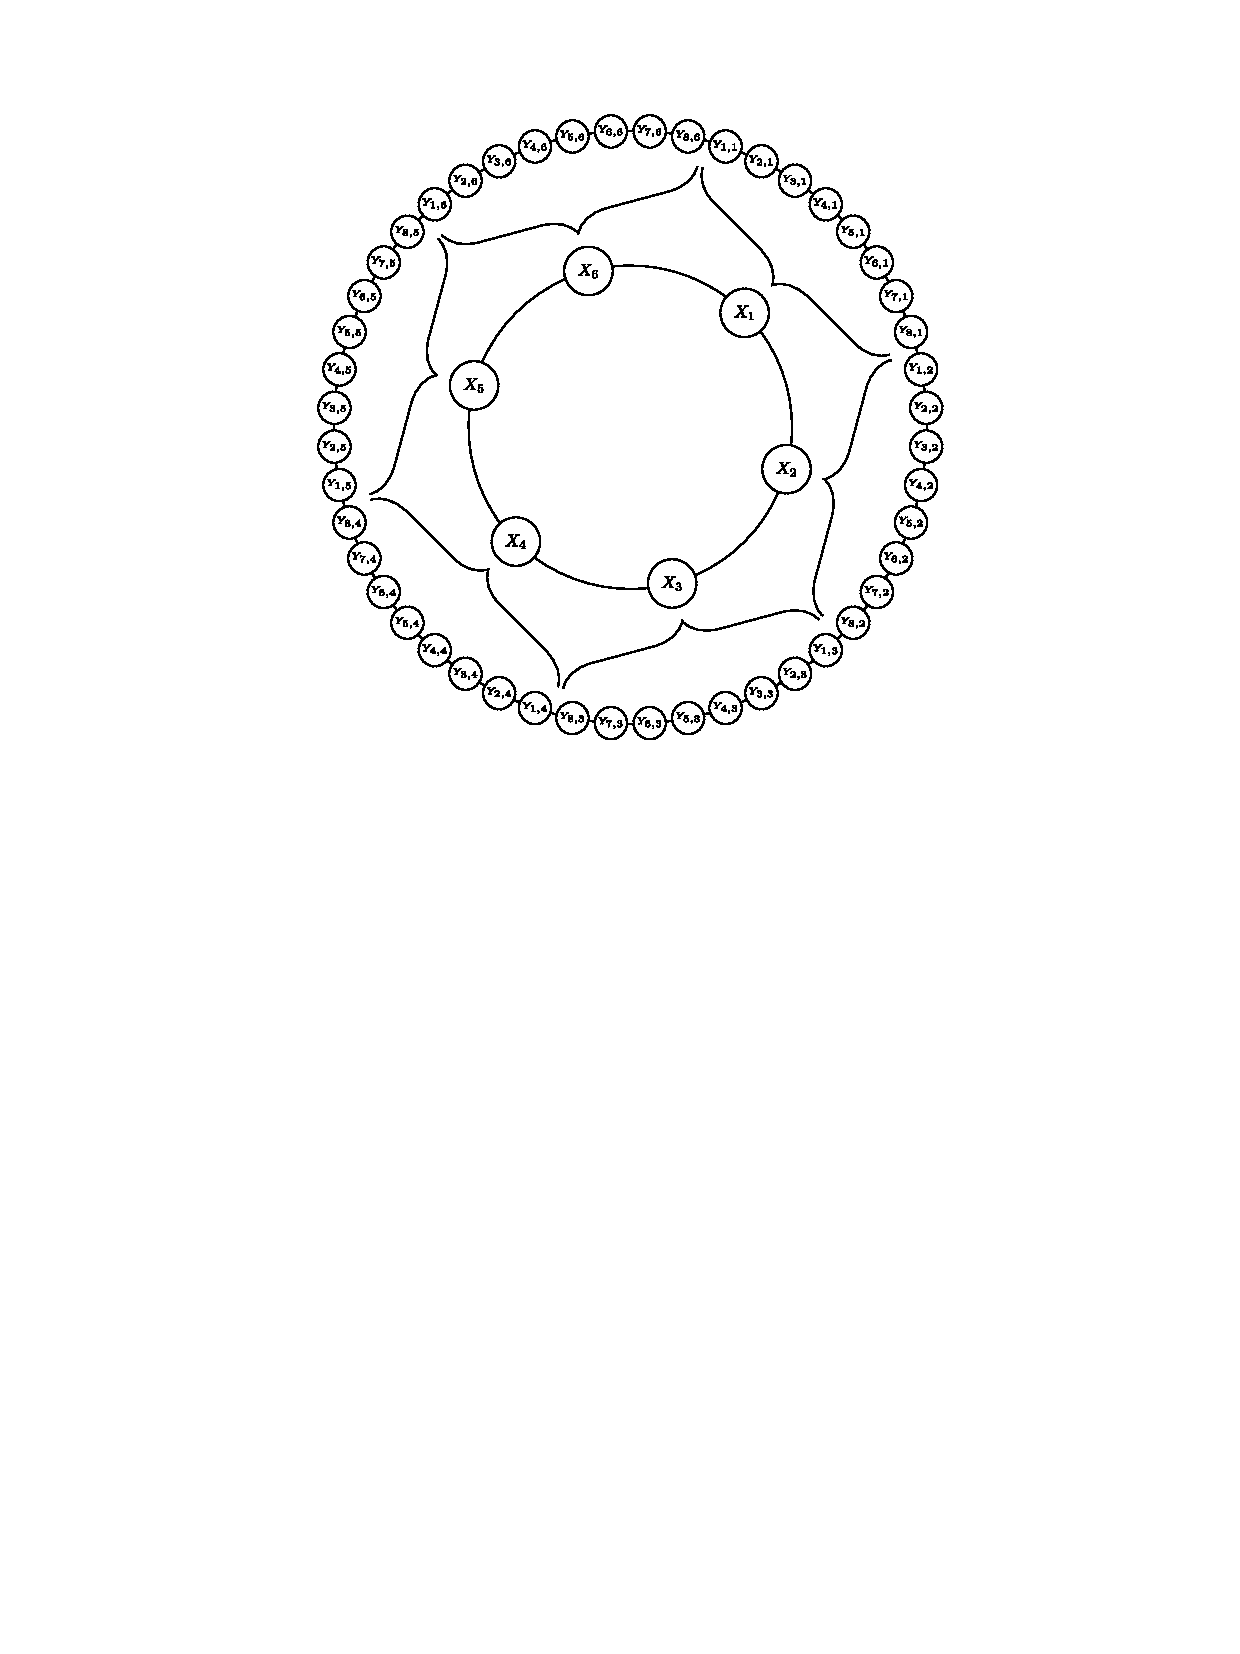
\includegraphics[width=0.7\linewidth]{figures/russell2017_L96_diagram.pdf}
    \caption{ Illustration of the periodic arrangement of the L96 variables,
        with the slow variables $X_k$ arranged in a circle. Each slow variable
        is coupled to a neighbouring subset of the similarly arranged fast
        variables $Y_{j,k}$. Reproduced from \textcite{russell2017}, Figure 1.
        }
    \label{fig:L96_diagram}
\end{figure}

As discussed in \cref{intro-sec:math}, the objective is to find $P_k(X_1,
\dots, X_K) \approx -(hc/b) \sum_{j=1}^J Y_{j,k}$ such that the solution of the
parametrised system
\begin{equation*}
    \diff{X_k}{t}
        = -X_{k-1} (X_{k-2} - X_{k+1}) - X_k + F + P_k(X_1, \dots, X_K)
\end{equation*}
approximates as accurately as possible the true $X_k$ obtained by solving
\cref{eqn:l96}. The simple form of L96 allows one to generate a training
dataset by numerically solving \cref{eqn:l96} and directly diagnosing the
unresolved tendency of $X_k$ as
\begin{equation} \label{eqn:l96_tendency}
    U_k(t) = \frac{X_k(t + \Delta t) - X_k(t)}{\Delta t}
        - \left[ -X_{k-1} (X_{k-2} - X_{k+1}) - X_k \right].
\end{equation}
As we shall see, it is usually assumed that $P_k$ depends only on $X_k$ (i.e.,
the parametrisation is \emph{local}) but may also depend on the value of $X_k$
at earlier times. The symmetry of \cref{eqn:l96} under shifts of the $k$ index
implies that all the $X_k$ have the same long-term statistics, so it suffices
to aggregate all the $U_k$ into a single training dataset and use the resulting
parametrisation for all the $X_k$ rather than constructing a separate
parametrisation for each variable.

\section{Statistical models} \label{sec:l96_statmodels} Constructing a
data-driven parametrisation scheme for L96 requires first choosing the
structure of the scheme and then using the training dataset to find the optimal
values of the associated free parameters. The simplest structure, popularised
in an influential paper by \textcite{wilks2005}, consists of a polynomial
regression of $U$ against $X$ as a deterministic base, modified by stochastic
noise. Wilks' scatterplot of $U$ and $X$ and quartic polynomial least-squares
regression, shown in \cref{fig:wilks2005_regression}, confirm that such a
structure is reasonable.

\begin{figure}[ht]
    \centering
    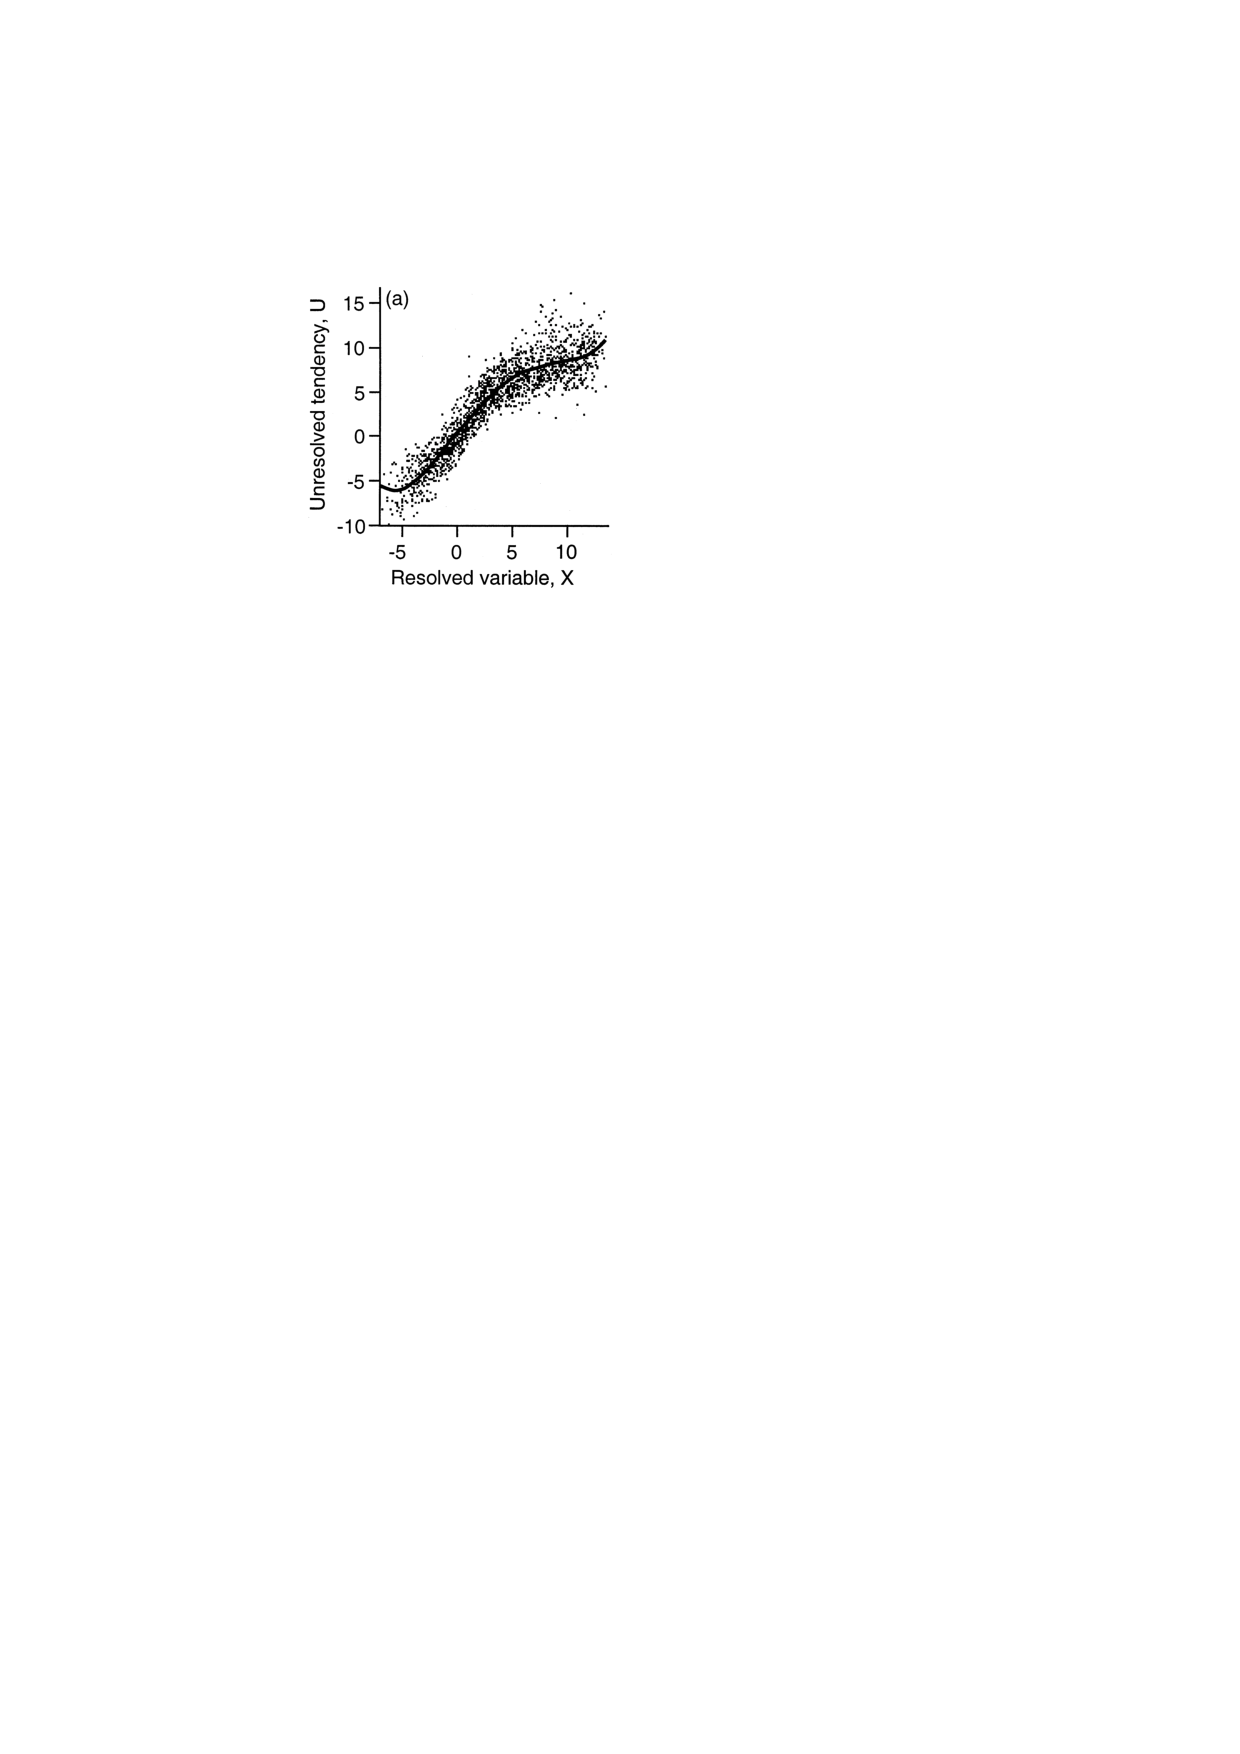
\includegraphics[width=0.3\linewidth]{figures/wilks2005_regression.pdf}
    \caption{ Scatterplot of unresolved tendencies $U$ against large-scale
        variables $X$ in L96 (black dots), and corresponding quartic polynomial
        least-squares regression (black line). Data are for forcing $F=18$.
        Reproduced from Figure 2a of \textcite{wilks2005}. }
    \label{fig:wilks2005_regression}
\end{figure}

Denote the deterministic polynomial part of the parametrisation by
$P_\mathrm{det}(X)$. Wilks' proposal was to then model the residuals as an
additive, mean-zero noise term $e(t)$, independent of $X$ and updated at each
time step, so that
\begin{equation} \label{eqn:l96_additive}
    P(X) = P_\mathrm{det}(X) + e(t).
\end{equation}
\textcite{arnold2013} and later \textcite{christensen2015} considered the SPPT
method (see \cref{intro-sec:stochastic}), where instead
\begin{equation} \label{eqn:l96_sppt}
    P(X) = [1 + e(t)] P_\mathrm{det}(X).
\end{equation}
The most common form for $e(t)$ in both \cref{eqn:l96_additive,eqn:l96_sppt} is
that of a \emph{first-order autoregressive} or AR(1) model
\begin{equation} \label{eqn:ar1}
    e(t) = \phi e(t - \Delta t) + \sigma z
\end{equation}
where $\phi \in [0,1]$ and $\sigma  \geq 0$ are constants and $z$ is drawn
independently from the standard normal distribution at each time step. The
AR(1) model introduces memory by having $e(t)$ relax from its value at the
previous time step towards zero, while also adding independent random jumps
with standard deviation $\sigma$. AR(1) noise is commonly also referred to as
\emph{red} noise. The two important special cases of an AR(1) model are $\phi =
0$, which reduces $e(t)$ to white noise without memory, and $\phi = \sigma =
0$, which results in a deterministic parametrisation $P(X) =
P_\mathrm{det}(X)$. The best estimates of $\phi$ and $\sigma$ are
straightforwardly obtained by examining the autocorrelation and standard
deviation of the residual time series $U(t) - P_\mathrm{det}(X(t))$ in the
training dataset (see \textcite{arnold2013} and \textcite[Chapter 9]{wilks2011}
for details).

It must be noted that the additive and SPPT schemes
\cref{eqn:l96_additive,eqn:l96_sppt} are inherently limited by their simple
form. The additive scheme assumes that the variance of the unresolved tendency
is independent of the value of $X$, and SPPT implies that the variance vanishes
when $P_\mathrm{det}(X)=0$. Inspection of \cref{fig:wilks2005_regression}
indicates that neither of these conditions is strictly satisfied.
\textcite{arnold2013} therefore proposed two possible modifications of
\cref{eqn:l96_additive}, with the standard deviation of $e(t)$ being a linear
function of either $|X(t)|$ or $|P_\mathrm{det}(X(t))|$.

Other studies have experimented with more complex statistical models for the
unresolved tendencies. \textcite{chorin2015} tested NARMAX (nonlinear
autoregression moving average with exogenous inputs), a model which represents
the tendency as a function of (i) the tendencies estimated at previous time
steps (autoregression), (ii) the current and previous values of $X$ (nonlinear;
exogenous data), (iii) independent Gaussian noise and (iv) the previous values
of the Gaussian noise (moving average). The motivation for NARMAX is that it
may be able to capture more complex relationships and memory effects by using
more predictors and free parameters. \textcite{crommelin2008,kwasniok2012} used
Markov chain models, which approximate the continuous range of possible
unresolved tendencies $U$ for a given $X$ by a discrete set of allowed states.
The model transitions from state to state according to a set of probabilities
that depend on $X$ and are estimated from the training dataset. The latest
studies have tested machine learning algorithms for L96, reflecting the
increasing research interest in ML-based parametrisation schemes for GCMs (see
\cref{intro-sec:data_driven}). \textcite{gagne2020} used generative adversarial
networks (GANs), which involve pairs of competing neural networks and have the
advantage of being stochastic with no need for \emph{ad hoc} perturbations.
\textcite{bhouri2023} used deterministic but memory-based neural networks
trained to directly optimise short-term forecast accuracy without requiring the
calculation of the unresolved tendencies $U$ in the training dataset.


\section{Evaluating parametrisation performance}
After choosing and fitting a parametrisation scheme, the next step is to assess
its performance. It is important to recognise that there are several contexts
in which one might want a parametrisation to perform well. The first important
distinction is between \emph{offline} and \emph{online} testing. Offline
testing involves feeding large-scale states into the parametrisation scheme
from a pre-computed test dataset that was not used for training (such as a new
high-resolution simulation) and measuring the level of agreement between the
tendencies predicted by the scheme and the true tendencies. Online testing, on
the other hand, involves coupling the parametrisation scheme into the host
model and comparing the output of the parametrised model to the corresponding
``truth'' solution (which might be the output of a high-resolution
unparametrised model). Online performance can further be assessed for
short-term (``weather'') forecasts or long-term (``climate'') predictions. The
reliability of ensemble forecasts (see \cref{intro-sec:stochastic}) must also
be determined. As we shall see, the extent to which good performance in more
than one category is achievable is a topic of ongoing research.

\subsection{Offline testing}
Offline testing is rarely documented in the L96 literature because it is
somewhat more straightforward than online testing. The aim is to ensure that
the parametrisation scheme accurately captures the distribution of unresolved
tendencies that exist in the true solution. \textcite{gagne2020} achieved this
by integrating the full system \cref{eqn:l96} to obtain a test dataset and
estimating the time-aggregated probability density functions (PDFs) of the true
unresolved tendencies \cref{eqn:l96_tendency} and the tendencies predicted by
the parametrisation schemes. They then expressed the difference between these
distributions as a scalar quantity using the Hellinger distance, defined for
two PDFs $p$ and $q$ by
\begin{equation} \label{eqn:hellinger}
    H(p,q) = \frac{1}{2} \int \mathrm{d}x
        \left( \sqrt{p(x)} - \sqrt{q(x)} \right)^2.
\end{equation}

\subsection{Forecast performance}
When evaluating online forecast accuracy for L96, studies are primarily
concerned with the agreement between a ``truth'' (or verification) solution of
\cref{eqn:l96} and the mean of an ensemble of independently realised,
stochastically parametrised forecasts starting from the same or nearby initial
conditions. This reflects standard practice in operational numerical weather
prediction. A standard approach is to calculate the root mean square error
(RMSE)
\begin{equation*}
    \mathrm{RMSE}(t) = \left( \left\langle
        \sum_k (X_k^\text{ens}(t) - X_k^\text{ver}(t))^2
    \right\rangle \right)^{1/2}
\end{equation*}
between the ensemble mean forecast $X_k^\text{ens}(t)$ and the verification
$X_k^\text{ver}(t)$, where the mean $\langle \cdot \rangle$ is taken over many
forecast-verification pairs with a range of initial conditions
\parencite{crommelin2008,gagne2020}.

An alternative for single-integration (non-ensemble) forecasts is to take the
mean over time, from the initial time up to time $t$ \parencite{bhouri2023}.
Another accuracy metric is the anomaly correlation (ANCR), which is the Pearson
correlation coefficient
\begin{equation*}
    \mathrm{ANCR}(t) = \left\langle
        \frac{
            \sum_k A_k^\text{ens}(t) A_k^\text{ver}(t)
        }{
            \left[
                \left( \sum_k A_k^\text{ens}(t)^2 \right)
                \left( \sum_k A_k^\text{ver}(t)^2 \right)
            \right]^{1/2}
        }
    \right\rangle
\end{equation*}
between the forecast anomaly $A_k^\text{ens}(t) = X_k^\text{ens}(t) - \langle
X_k^\text{ver}(t) \rangle_t$ and the verification anomaly $A_k^\text{ver}(t) =
X_k^\text{ver}(t) - \langle X_k^\text{ver}(t) \rangle_t$, again averaged over
forecast-verification pairs \parencite{crommelin2008}. Other studies
\parencite{kwasniok2012,arnold2013} have used more complex skill scores to
assess forecast accuracy.

Recall from \cref{intro-sec:stochastic} that an ensemble forecast is said to be
reliable if the spread of the ensemble members is representative of the range
of weather states that could possibly be realised, given the initial condition
uncertainty and model errors. In the context of L96, there are two ways to
measure reliabilty. The first \parencite{wilks2005,crommelin2008,kwasniok2012}
is to sort the states $X_k$ of the ensemble members at the chosen lead time
from largest to smallest (or vice versa), and find the rank that the truth
state would occupy within the list. The ranks from many ensemble forecasts are
aggregated and their distribution plotted on a \emph{rank histogram}, which
should ideally be uniform for a well-dispersed ensemble. A U-shaped rank
histogram indicates underdispersion; that is, the truth too frequently lies at
the extreme ends of or outside the ensemble. An inverted U shape indicates the
opposite (overdispersion). Another method is to simply compare the ensemble
standard deviation and the RMSE, which should be roughly equal for a reliable
forecast \parencite{arnold2013,gagne2020}.

\subsection{Climate prediction performance}
There are several classes of metrics and methods available for assessing the
accuracy of long-term climate predictions made by parametrised L96 models. The
simplest is to compare the low-order moments (mean, variance) of the long-term
distributions of $X$ between the parametrised and truth solutions. However, it
is often the case for the relatively simple L96 model that parametrised models
reproduce these moments quite accurately \parencite{wilks2005}, motivating
comparison of the entire PDFs---a more stringent test. In addition to visual
comparison of the PDFs, one can use scalar measures such as the Hellinger
distance \cref{eqn:hellinger} \parencite{arnold2013,gagne2020} and the
Kolmogorov-Smirnov statistic
\begin{equation*}
    D_n = \max_X |\Psi_\mathrm{true}(X) - \Psi_\mathrm{model}(X)|,
\end{equation*}
which is the maximum absolute difference between the cumulative distribution
functions $\Psi$ of $X$ in the truth and parametrised models
\parencite{wilks2005,chorin2015,kwasniok2012}. As a diagnostic tool, it is also
possible to compare the joint distributions of $X$ and the unresolved tendency
$U$ between the truth and parametrised models \parencite{gagne2020}.

Another approach is to study the correlation and spectral properties of $X$. In
the time domain, one can compute the autocorrelation function $\langle X_k(t)
X_k(t + \tau) \rangle_{t,k}$ or the cross-correlation $\langle X_k(t) X_{k+1}(t
+ \tau) \rangle_{t,k}$ between neighbouring variables and compare these to
their truth counterparts
\parencite{crommelin2008,kwasniok2012,chorin2015,gagne2020}.
\textcite{gagne2020} applied the continuous wavelet transform (CWT) to the
$X(t)$ time series to measure the amount of power in the signal as a function
of oscillation period. Similar analyses may be performed in ``space'' by
computing the autocorrelation $\langle X_k(t) X_{k+n}(t) \rangle_{t,k}$ with
respect to shifts in the $k$ index \parencite{gagne2020} or by taking a
discrete Fourier transform of $X_k$ with respect to $k$ and deriving wavenumber
statistics \parencite{crommelin2008,kwasniok2012}.


\section{Lessons learnt from Lorenz '96}
Now that the statistical models and analysis techniques for L96 parametrisation
have been surveyed, I shall review the results of previous studies, focusing on
key conclusions that have potential implications for more complex dynamical
systems. The common objective in many studies has been to determine the value
added by stochasticity and memory. The general consensus is that
parametrisations with white noise outperform purely deterministic ones, and
that adding memory via red noise or dependence on past large-scale states gives
a further advantage over white noise
\parencite{wilks2005,arnold2013,gagne2020}. The advantages of stochasticity and
memory include improvements in the skill and reliability of ensemble forecasts
and in the accuracy of climatological probability distributions.
\textcite{arnold2013} additionally found that parametrisations with
state-dependent noise have the potential to produce more skilful forecasts than
those with state-independent additive noise. This was only observed under
conditions of small time-scale separation between the resolved and unresolved
variables (i.e., $c \sim 1$ in \cref{eqn:l96}); it appeared that simple
additive noise was sufficient for larger scale separation. A representative
illustration of the conclusions for short-term forecasting and climate
prediction are respectively given by Figures 6 and 10 of
\citeauthor{arnold2013}, which are reproduced here as
\cref{fig:arnold_fig6,fig:arnold_fig10}.

\begin{figure}[ht]
    \centering
    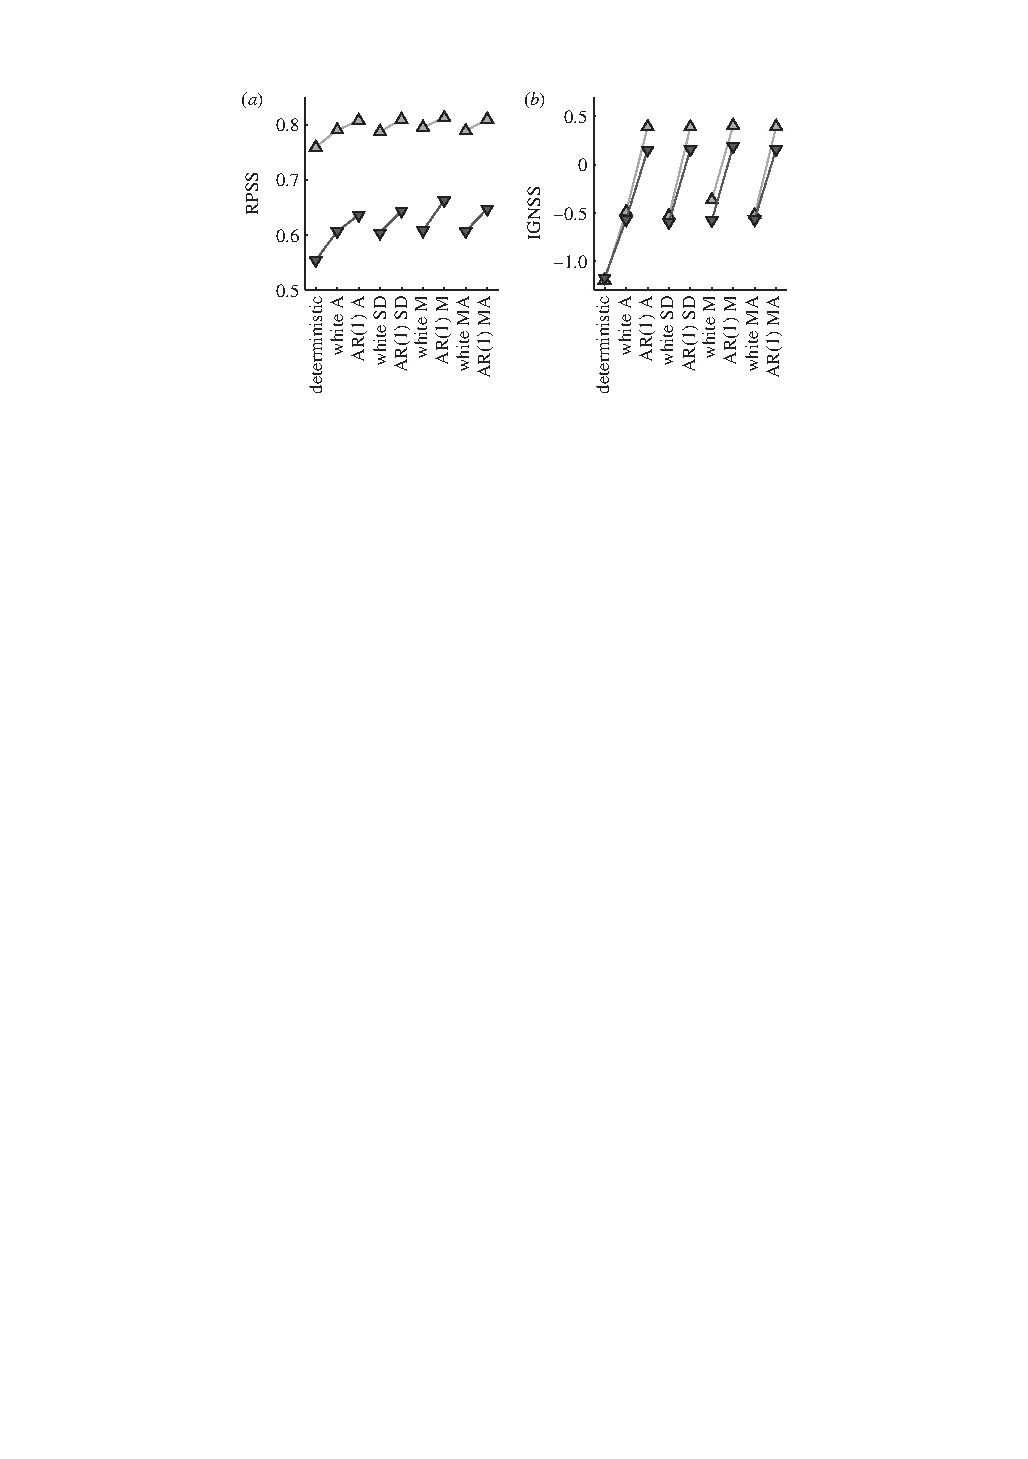
\includegraphics[width=0.6\linewidth]{figures/arnold2013_fig6.pdf}
    \caption{ Reproduction of Figure 6 by \textcite{arnold2013}, showing a
        comparison of ensemble forecast skill for parametrisations with
        different types of noise. Skill is measured by the ranked probability
        skill score (RPSS; panel (a)) and ignorance skill score (IGNSS; panel
        (b)); higher values indicate better skill. The deterministic
        parametrisation is a cubic polynomial regression and added noise is
        either white or generated by an AR(1) process. Acronyms indicate the
        method used to introduce the noise; A = ``additive'', SD =
        ``state-dependent'' (noise standard deviation a linear function of
        $|X|$), M = ``multiplicative'' (SPPT) and MA = ``multiplicative and
        additive'' (noise standard deviation a linear function of
        $|P_\mathrm{det}(X)|$). Upright light grey triangles indicate results
        obtained under conditions of larger time scale separation ($c=10$ in
        \cref{eqn:l96}) and inverted dark grey triangles indicate smaller time
        scale separation ($c=4$). It is clear that schemes with white noise
        outperform deterministic ones, and schemes with AR(1) noise outperform
        whose with white noise. }
    \label{fig:arnold_fig6}
\end{figure}
\begin{figure}[H]
    \centering
    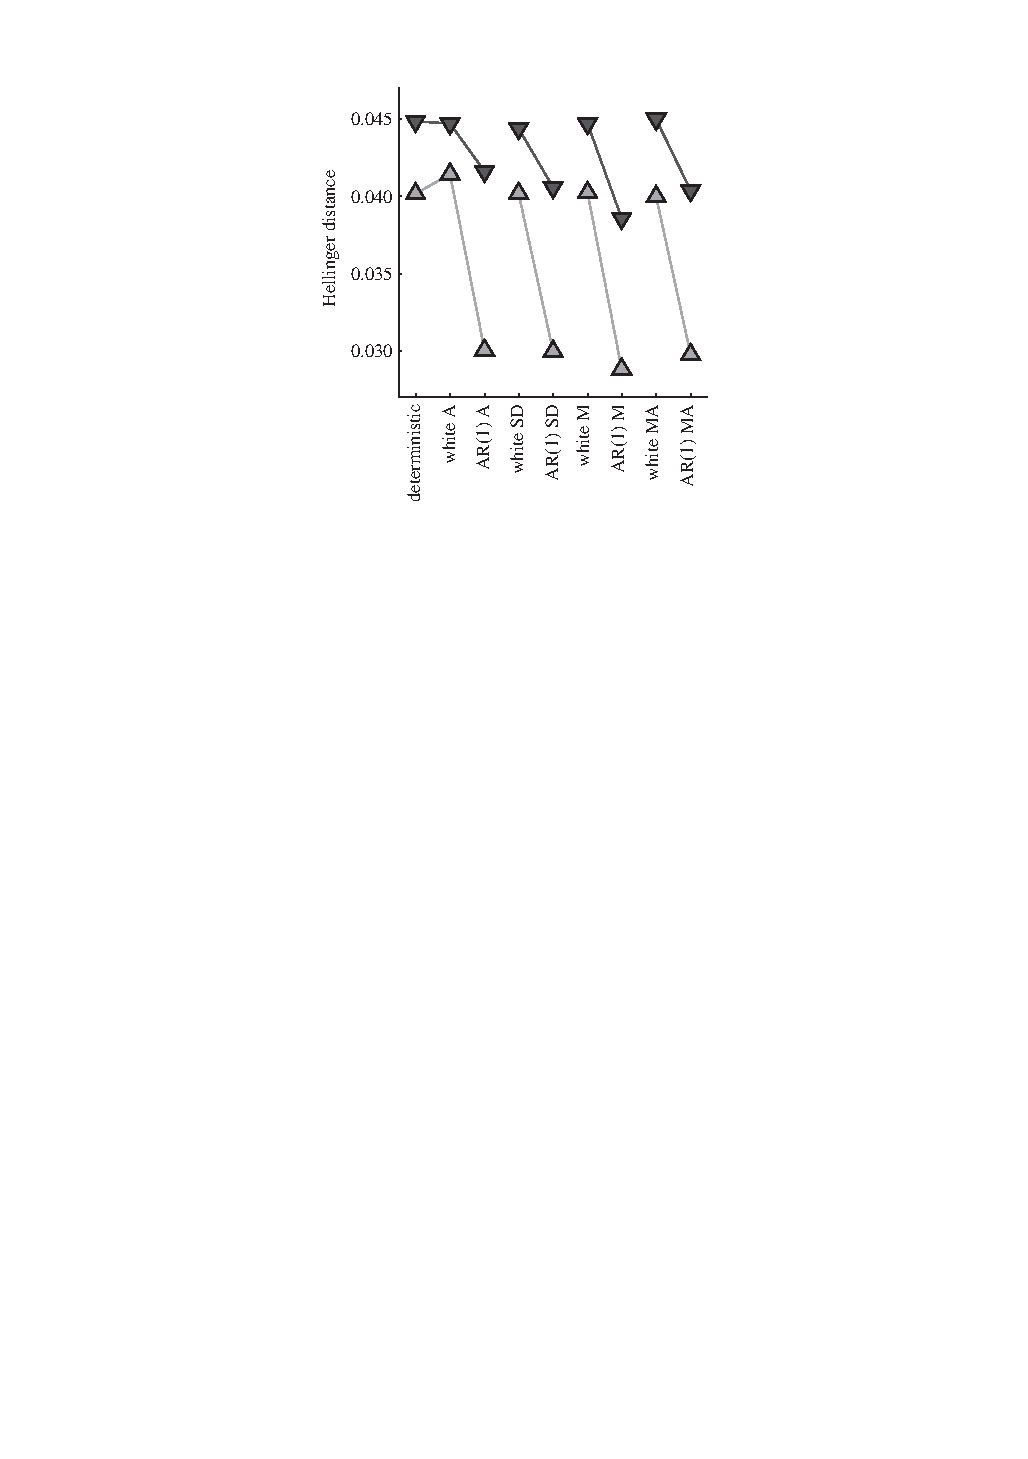
\includegraphics[width=0.4\linewidth]{figures/arnold2013_fig10.pdf}
    \caption{ Reproduction of Figure 10 by \textcite{arnold2013}, comparing the
        accuracy with which parametrisations with different types of noise
        reproduce the true climatological PDFs of the resolved variables.
        Accuracy is measured by the Hellinger distance between the modelled and
        true PDFs; lower values indicate higher accuracy. The labels on the
        horizontal axis and the markers have the same meaning that they do in
        \cref{fig:arnold_fig6}. A clear improvement in accuracy is given by the
        schemes with AR(1) noise. }
    \label{fig:arnold_fig10}
\end{figure}

Some studies have obtained results that conflict with the aforementioned
consensus. Firstly \textcite{arnold2013} found no appreciable difference in
climatological PDF accuracy between their white noise and deterministic
schemes; this is evident in \cref{fig:arnold_fig10}. Analogously,
\textcite{christensen2015} similarly found no significant difference between
white noise and deterministic schemes in terms of their ability to reproduce
regime behaviour and predict the system's response to changes in the external
forcing parameter $F$. \textcite{gagne2020}, who constructed parametrisations
using generative adversarial networks, came to the unexpected conclusion that
using temporally correlated red noise may degrade the accuracy of ensemble
forecasts via an accumulation of noise-induced error and have little benefit
over white noise for climate prediction accuracy.

Several authors have postulated general interpretations of these results that
may be relevant to the parametrisation problem in dynamical systems beyond L96.
\textcite{arnold2013} attributed the apparent superiority of memory-based
parametrisations to a potential for subgrid-scale processes to influence the
resolved state on scales much larger than the grid scale at which the host
model is truncated; memory captures this spatial and temporal correlation or
persistence. \textcite{christensen2015} agreed with this assessment on the
basis of their results. They also argued that the persistence of correlated
noise is necessary to drive regime transitions that would otherwise be
underrepresented. Observing that stochastic parametrisation improved the
prediction of responses to changes in forcing, they further argued that
stochastic data-driven parametrisations are generally more likely to function
well in changed climate conditions outside the range of their training
datasets.


\section{Open questions and the case for more complex dynamical systems}
To conclude this section on data-driven parametrisation for L96, I will draw on
the key messages and conclusions in the literature to motivate further research
of the same kind in models of intermediate complexity.

Generally speaking, many parametrisation approaches of varying complexity have
shown promise when applied to L96; all the studies mentioned in
\cref{sec:l96_statmodels} were able to construct a scheme that reproduced the
properties of interest without egregious errors. Indeed, some of the more
recent and complex approaches have shown only marginal improvements over the
original regression-based approach introduced by \textcite{wilks2005}.
\textcite{gagne2020} attributed this to the simplicity of L96, which only
considers the evolution of a single field in one discrete spatial dimension.
There is hope that applying the L96 methods to dynamical systems with more
prognostic variables, spatial dimensions and degrees of freedom may reveal
deficiencies that were inconsequential in L96 and thus give researchers more
discriminative power in choosing approaches for application to full GCMs.

Several specific findings in L96 studies raise other questions that also
motivate a change of focus to more complex dynamical systems. The first is the
observation by \textcite{crommelin2008} that the advantage of their conditional
Markov chain parametrisation over the regression-based approach was greatest
under conditions of small time-scale separation and diminished with increasing
scale separation. \textcite{arnold2013} drew a similar conclusion regarding the
difference between stochastic and deterministic regression-based schemes. These
findings are consistent with the expectation that the net effect of
subgrid-scale processes should become increasingly unpredictable as resolution
increases and the size of the sample of small-scale events decreases (see
\cref{intro-sec:traditional}). This is another piece of evidence that more
realistic fluid models, which do not have such a clean separation between
``resolved'' and ``unresolved'' variables, will be more discriminating and
allow the best approaches to show their full potential.

An open question of importance for real-world modelling concerns the extent to
which parametrisation schemes that result in accurate weather forecasts tend
can be expected to also produce accurate climate predictions
\parencite{christensen2019}. Another asks whether a scheme's offline
performance is a good indicator of its online performance once coupled into a
model. \textcite{gagne2020} addressed these questions by testing a collection
of GAN parametrisations with different predictors and types of noise (see
\cref{fig:gagne_fig11}), with the results suggesting an affirmative answer for
the former and a negative answer for the latter. The verification of these
conclusions would be a worthwhile goal for further research using other
dynamical systems. Other possible goals could be to more clearly assess the
ability of data-driven parametrisation schemes to adapt to unseen climate
conditions \parencite{christensen2015} and to explore and exploit the potential
for data-driven schemes to correct numerical errors in addition to modelling
unresolved processes \parencite{bhouri2023}.

\begin{figure}[ht]
    \centering
    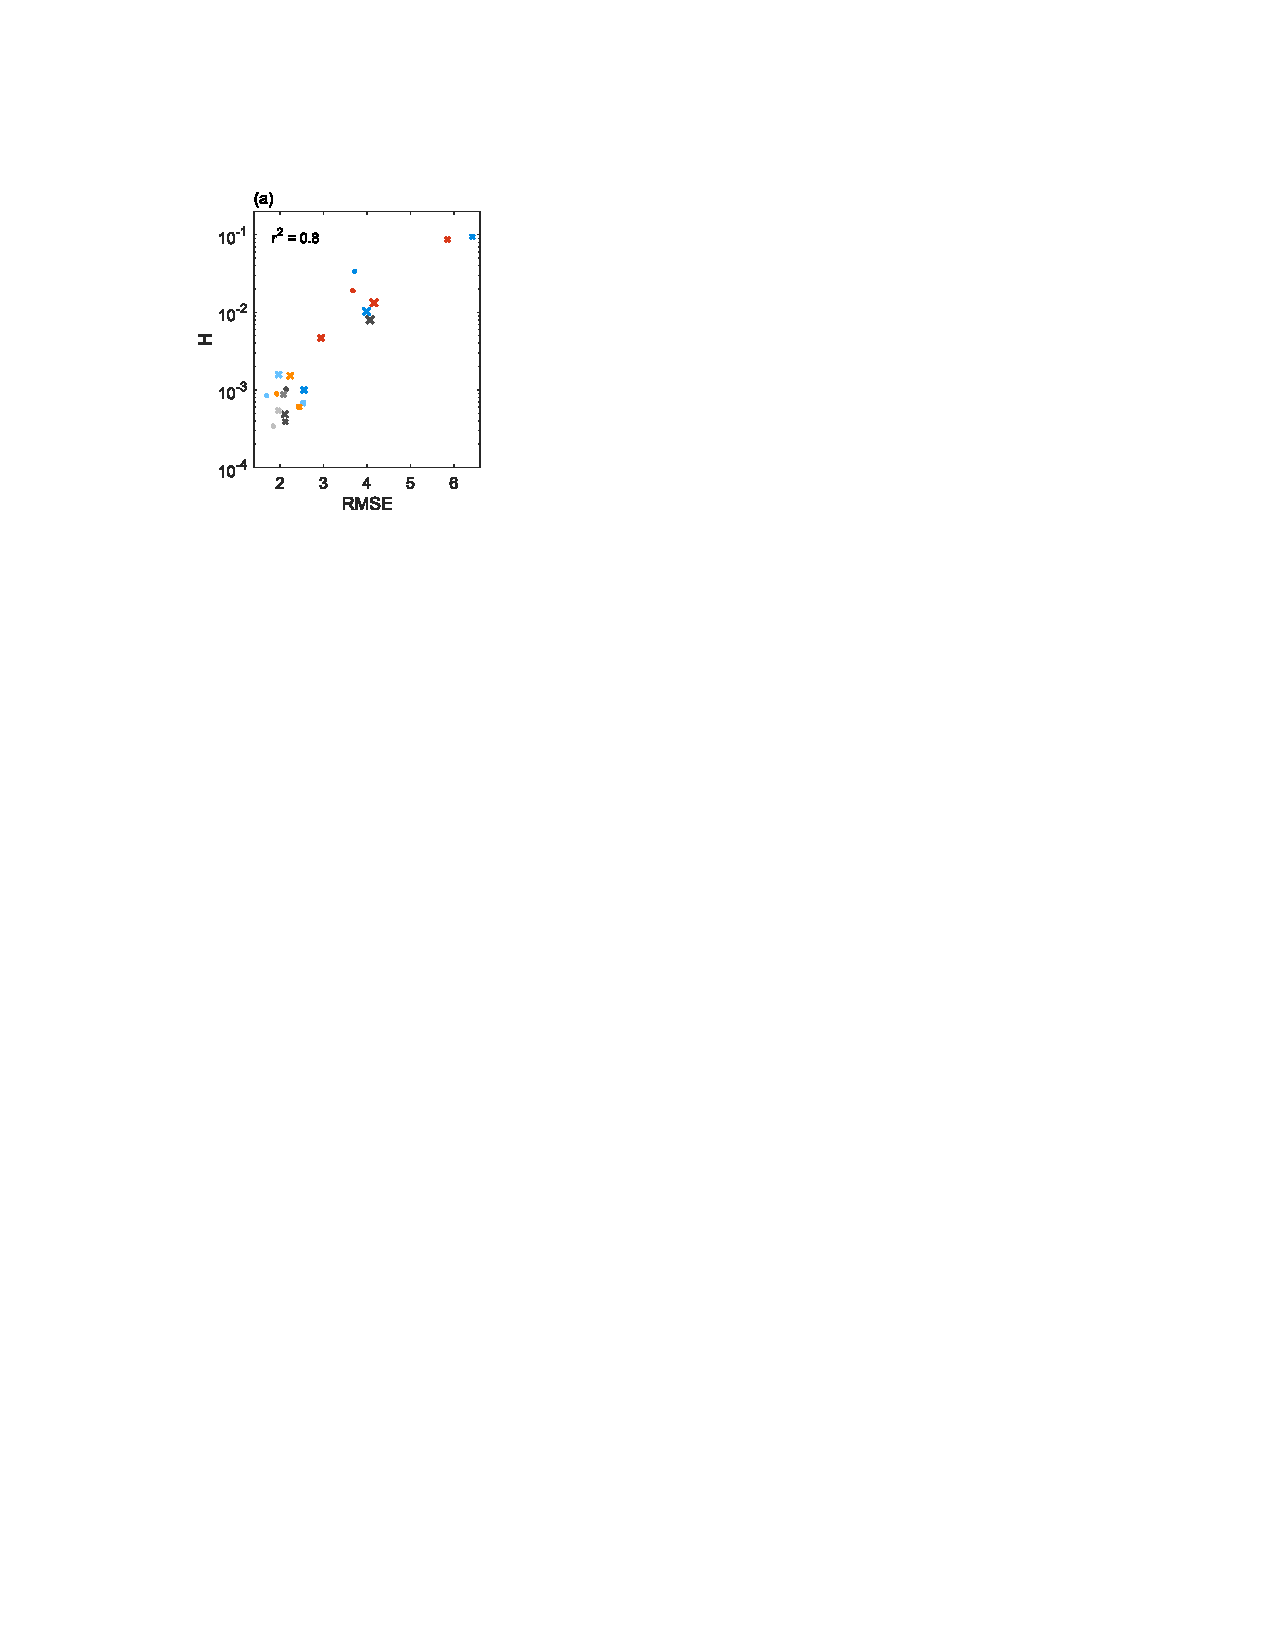
\includegraphics[width=0.3\linewidth]{figures/gagne_fig11a.pdf}%
    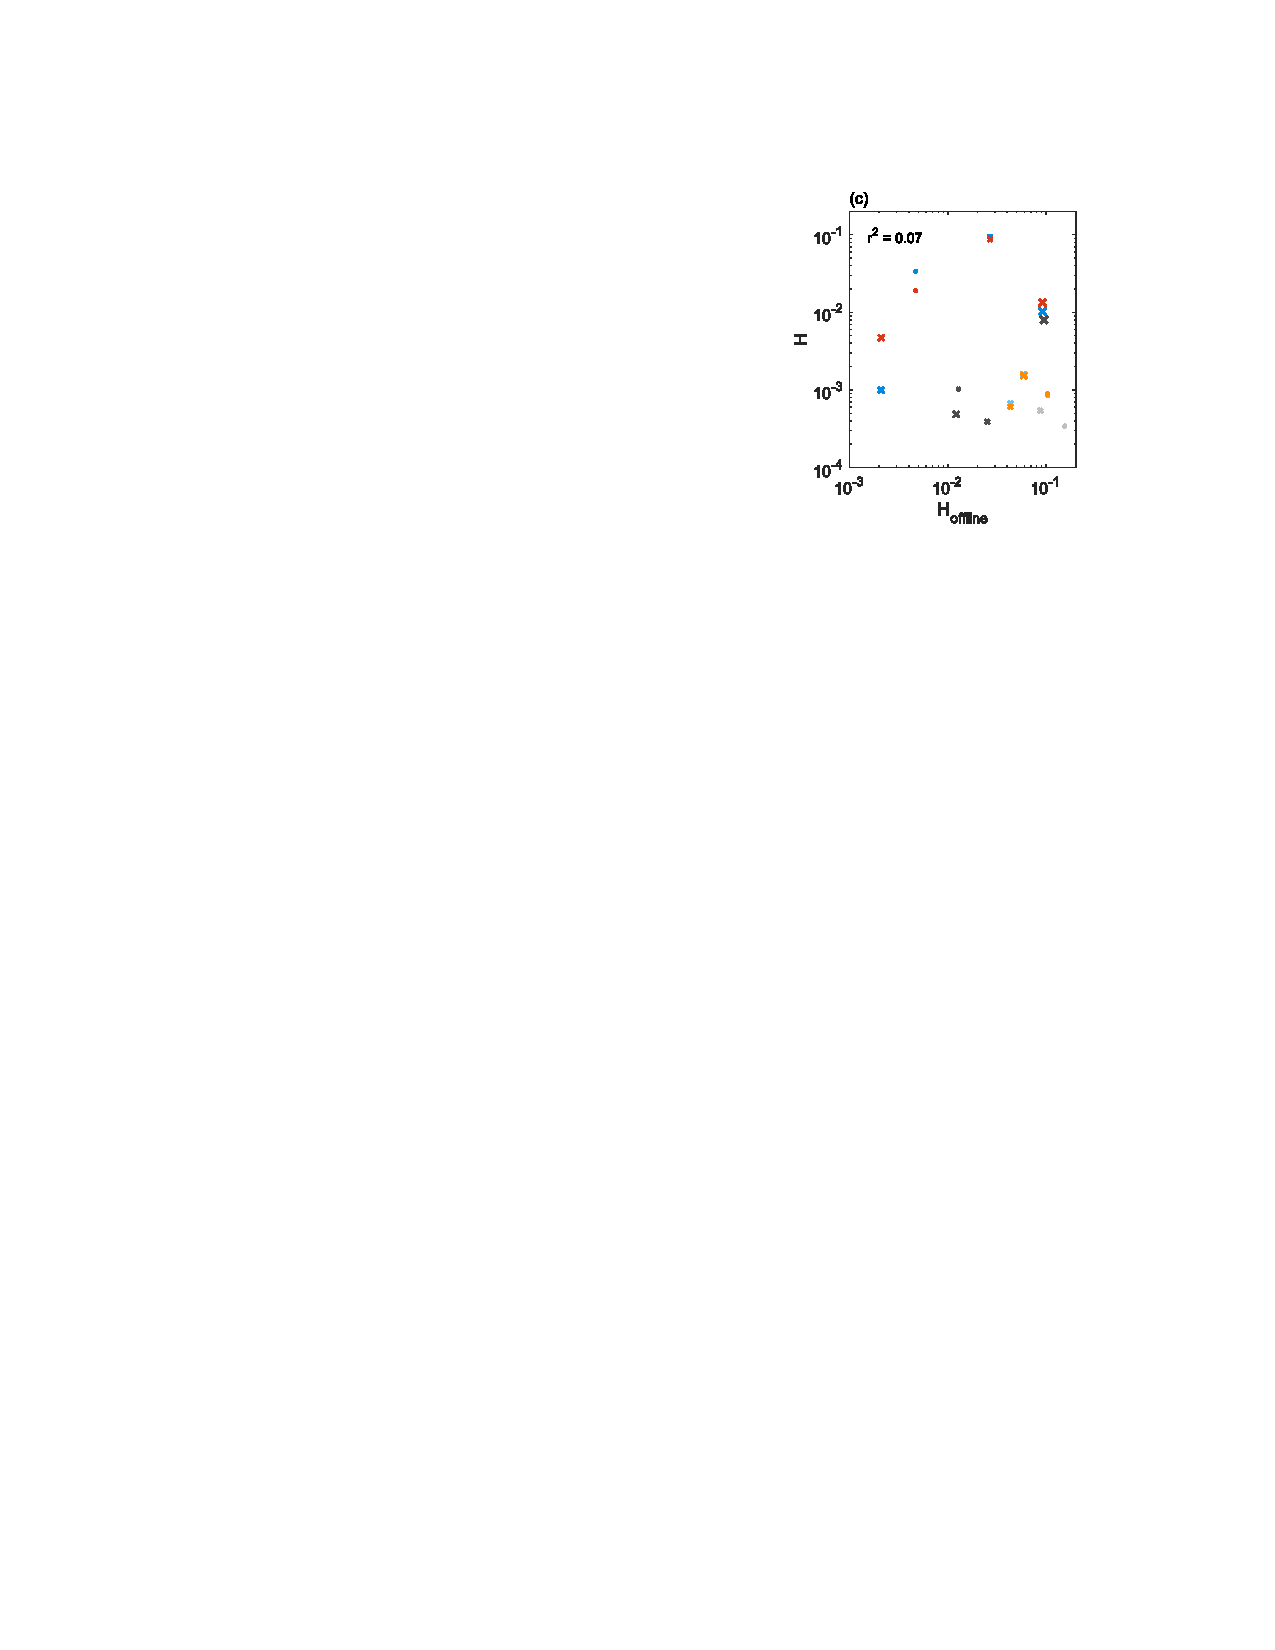
\includegraphics[width=0.3\linewidth]{figures/gagne_fig11c.pdf}
    \caption{ Reproduction of Figures 11a and 11c by \textcite{gagne2020}.
        Panel (a) compares ensemble mean weather forecast accuracy (measured by
        RMSE) to climatological PDF accuracy (measured by the Hellinger
        distance $H$) for a collection of GAN parametrisations with different
        predictors and types of noise. Panel (c) performs a similar comparison
        with offline performance (measured by the Hellinger distance between
        the PDFs of the true and predicted tendencies) taking the place of
        RMSE. }
    \label{fig:gagne_fig11}
\end{figure}


\section{Beyond Lorenz '96}
The transition from L96 to more complex systems necessarily gives rise to
several technicalities that must be addressed. The most pressing of these is
the fact that increasing the number of degrees of freedom in the host model
will greatly increase the number of predictors available for parametrisations
to use. Models with more than one prognostic variable will also require
separate parametrisations for each one. Without judicious simplifications, the
problem of constructing a rigorous data-driven parametrisation will quickly
become intractable. \textcite{crommelin2008} give an insightful discussion of
this issue as it relates to Markov chain parametrisations.

Another complication is that the ``spatial'' dimension in L96 is discrete,
while the dynamical systems being parametrised in weather and climate modelling
(i.e., fluid flows) have continuous spatial dimensions. While it is well
established that there is little benefit in using stochastic parametrisations
with spatially correlated noise for L96, spatial correlation is expected to be
a much more important consideration in spatially continuous systems
\parencite{arnold2013}. One might also ask whether it will be beneficial to
construct spatially nonlocal schemes where the tendency predicted at each point
also depends on the values of the large-scale variables at neighbouring points
(potentially capturing the gradients of these variables).


\ifSubfilesClassLoaded{%
    \emergencystretch=5em
    \printbibliography{}
}{}

\end{document}
